\section{Experiment Setup}\label{sec:experimentsetup}
The experimental evaluation is done by help of several experiments on the two versions of the CoAP protocol. For these experiments different setups are made, all based on the IoTivity framework v1.1.0 running on two Linux (Ubuntu) machines as illustrated in \figurename \ref{fig:setup}. These two machines are both wireless coupled to a local network via a router. 

The first setup is for CoAP and uses two applications. These are, a simple IoTivity client and a server application. Both applications are developed in C++ and uses CoAP as an application protocol.

The second setup is for CoAP over TCP and also uses two applications. These are, a simple IoTivity client application developed in C++ and a simple IoTivity server application developed in Java. Both applications uses CoAP over TCP as an application protocol.

\begin{figure}[bht]
	\centering
	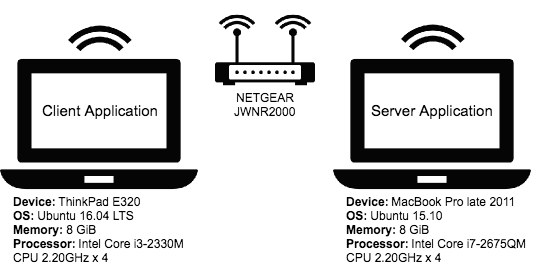
\includegraphics[width=3.5in]{gfx/setupa}
	\caption{The testbed.}
	\label{fig:setup}
\end{figure}

The test case for the experiments is meant to represent a constrained device, acting as a client, updating the temperature on a cloud server with a specific interval of time. 

Linux is chosen to represent a constrained device as it is necessary to be able to easily monitor the communication traffic between the client and the server from the client side of view.
%Wireshark....
The Wireshark network protocol analyzer tool is used for the monitoring.





%\textbf{Memory consumption}\\
%Flyt den del til et afsnit med prototype implementation (før resultaterne)
%How much memory usage...
